\section{Performances de la Programmation Linéaire Mixte}
\label{sec:expe_PLNE}
Dans ce paragraphe, nous détaillons les résultats expérimentaux
obtenus par les modèles présentés dans le
chapitre~\ref{sec:PLNE_CECSP} et l'influence des techniques de
renforcement présentées dans ce même chapitre. Nous commençons, dans
un premier temps, par présenter les résultats obtenus pour le modèle
indexé par le temps puis nous détaillerons les résultats des modèles à événement.

\subsection{Modèles indexés par le temps}
Dans ce paragraphe, nous décrivons les performances du modèle indexé
par le temps pour le \CECSP. Les expérimentations ont été conduites
sur les quatre familles d'instances présentées dans le
paragraphe~\ref{sec:instance_CECSP} et avec une limite de temps de 100
secondes. Le modèle, avec pour objectif la minimisation de la
consommation totale de ressource, est dans un premier temps utilisé
pour résoudre les instances. Dans un second temps, nous ajoutons les
inégalités issues du raisonnement énergétiques décrites dans le
paragraphe~\ref{sec:ER_TI}. Ces inégalités sont seulement ajouter au
n\oe ud racine de l'arbre de recherche. En effet, dû à leur grand
nombre ($5*|\I|*n$, avec $\I$ l'ensemble des intervalles d'intérêt du
raisonnement énergétique) , il est difficile, sans algorithme de
séparation, de les inclure dynamiquement pendant la recherche. Le
tableau~\ref{tab:TI_CECSP} présente ces résultats.

Dans ce tableau, nous avons comparé la qualité et le temps d'obtention
des premières solutions pour chaque famille d'instances et pour les
cas avec et sans coupes énergétiques. La qualité de la solution est
mesurée de la manière suivante: 
\[
  \text{gap}=100*\frac{|\text{Objectif final} - \text{Objectif } 1^{ère} \text{  Sol}|}{\text{Objectif final}}
\]
Nous avons aussi comparé le temps nécessaire à l'obtention de la
solution optimale (100 secondes si la solution trouvé n'est pas
optimale), la qualité de la solution, le nombre d'instances résolues
et le nombre d'entre elles résolues à l'optimal.

\begin{table}[!htb]
  \begin{center}\small
    \begin{tabularx}{\linewidth}{|Y|YY|YYYY|YY|YYYY|}
      \hline
      \multirow{2}{*}{\#act.} & \multicolumn{2}{c|}{$1^{ère}$ sol.}&
      \multicolumn{4}{c|}{final sol.} & \multicolumn{2}{c|}{$1^{ère}$ 
        sol.}&
      \multicolumn{4}{c|}{sol. finale} \\ 
      \cline{2-13} 
                               & tps(s) & gap & tps & gap  &  \%opt.&\%solv.&
                                                                 tps
                                                                 & gap
                                                                 &
                                                                 tps
                                                                 & gap
                                                                 &
                                                                 \%opt. &\%solv.  \\ 
      \hline
      \multicolumn{7}{|l|}{Famille 1} & \multicolumn{6}{|l|}{Famille 2}\\
      \hline
      \multicolumn{7}{|r|}{sans coupes énergétiques} & \multicolumn{6}{|r|}{sans coupes énergétiques}\\
      \hline  
      $10 $&$ 0,058 $&$ 38 $&$ 45 $&$ 2,9$ &$ 60 $&$ 100$ &$ 0,075 $&$ 24 $&$ 100 $&$ 5,6$ &$ 0 $&$ 100$ \\ 
      $20 $&$ 0,25 $&$ 17 $&$ 100 $&$ 8,4$ &$ 0 $&$ 100$ & $ 0,37 $&$ 8,8 $&$ 100 $&$ 6,5$ &$ 0 $&$ 100$\\ 
      $25 $&$ 0,88 $&$ 21 $&$ 100 $&$ 9,4$ &$ 0 $&$ 100$ &$ 2 $&$ 12 $&$ 100 $&$ 5,8$ &$ 0 $&$ 100$ \\ 
      $30 $&$ 1,3 $&$ 35 $&$ 100 $&$ 10$ &$ 0 $&$ 100$&$ 3,1 $&$ 14 $&$ 100 $&$ 6,3$ &$ 0 $&$ 100$  \\ 
      \hline 
      \multicolumn{7}{|r|}{avec coupes énergétiques à la racine} &  \multicolumn{6}{|r|}{avec coupes énergétiques à la racine}\\
      \hline
      $10 $&$ 0,064 $&$ 3,4 $&$ 60 $&$ 2,6$ &$ 40 $&$ 100$ &$ 0,074 $&$ 9 $&$ 100 $&$ 4,1$ &$ 0 $&$ 100$\\ 
      $20 $&$ 0,31 $&$ 18 $&$ 100 $&$ 8,7$ &$ 0 $&$ 100$& $ 0,65 $&$ 9,4 $&$ 100 $&$ 6,2$ &$ 0 $&$ 100$  \\ 
      $25 $&$ 0,63 $&$ 17 $&$ 100 $&$ 9,6$ &$ 0 $&$ 100$ &$ 1,9 $&$ 12 $&$ 100 $&$ 6$ &$ 0 $&$ 100$\\ 
      $30 $&$ 1,6 $&$ 18 $&$ 100 $&$ 10$ &$ 0 $&$ 100$ &$ 5,8 $&$ 11 $&$ 100 $&$ 6,3$ &$ 0 $&$ 100$ \\ 
      \hline   
      \multicolumn{7}{|l|}{Famille 3} &  \multicolumn{6}{|l|}{Famille 4}\\
      \hline
      \multicolumn{7}{|r|}{sans coupes énergétiques}&  \multicolumn{6}{|r|}{sans coupes énergétiques}\\
      \hline  
    $10 $&$ 0,064 $&$ 4,1 $&$ 64 $&$ 1,8$ &$ 40 $&$ 100$ &$ 0,037 $&$ 0 $&$ 0,037 $&$ 0$ &$ 100 $&$ 100$\\ 
$20 $&$ 2,8 $&$ 6,8 $&$ 100 $&$ 3,9$ &$ 0 $&$ 100$ &$ 0,61 $&$ 0,72 $&$ 0,63 $&$ 0$ &$ 100 $&$ 100$\\ 
$25 $&$ 17 $&$ 4,5 $&$ 100 $&$ 4,5$ &$ 0 $&$ 100$ &$ 1,5 $&$ 0,31 $&$ 1,5 $&$ 0$ &$ 100 $&$ 100$\\ 
$30 $&$ 24 $&$ 6,4 $&$ 100 $&$ 4,1$ &$ 0 $&$ 80$ &$ 4,8 $&$ 0,07 $&$ 15 $&$ 0$ &$ 89 $&$ 89$ \\ 
      \hline 
      \multicolumn{7}{|r|}{avec coupes énergétiques à la racine} & \multicolumn{6}{|r|}{avec coupes énergétiques à la racine}\\
      \hline
$10 $&$ 0,063 $&$ 3,4 $&$ 80 $&$ 1,8$ &$ 20 $&$ 100$&$ 0,045 $&$ 1,1 $&$ 0,046 $&$ 0$ &$ 100 $&$ 100$  \\ 
$20 $&$ 2,5 $&$ 6,7 $&$ 100 $&$ 3,8$ &$ 0 $&$ 100$ &$ 0,56 $&$ 0,64 $&$ 0,71 $&$ 0$ &$ 100 $&$ 100$  \\ 
$25 $&$ 18 $&$ 5,8 $&$ 100 $&$ 4,4$ &$ 0 $&$ 100$ &$ 2,6 $&$ 0,072 $&$ 2,9 $&$ 0$ &$ 100 $&$ 100$ \\ 
$30 $&$ 24 $&$ 7,6 $&$ 100 $&$ 4,2$ &$ 0 $&$ 70$ &$ 6,4 $&$ 0 $&$ 6,4 $&$ 0$ &$ 100 $&$ 100$\\ 
      \hline   
    \end{tabularx}
  \end{center}
  \caption{Résultats du PLNE indexé par le temps du \CECSP~avec et
    sans coupes énergétiques.} 
  \label{tab:TI_CECSP}
\end{table}

Les résultats présentés dans le tableau~\ref{tab:TI_CECSP} montrent
que, dans la majorité des cas, le modèle avec les coupes énergétiques
obtient une première solution de meilleure qualité que celle obtenue
sans ces coupes. De plus, le temps de calcul de cette première
solution, bien que légèrement plus élevé dans le cas des coupés
énergétiques, est du même ordre de grandeur dans les deux cas.

Cependant, sauf dans le cas des instances à 30 activités de la Famille
4 où l'ajout des coupes permet un gain en termes de performances, les
coupes énergétiques ne produisent pas de gain significatif, ni en
termes de qualité de solution, ni en termes de temps de résolution. 

Malgré tout, les performances relatives des coupes énergétiques pour
le calcul des premières solutions pousse à poursuivre cette
investigation. La mise en place en place d'un algorithme de séparation
permettant de trouver les meilleures coupes à ajouter à chaque n\oe ud
de l'arbre de recherche devient donc une direction de recherche
encourageante dans un futur proche. 

\subsection{Modèles à événements}

Ce paragraphe, dédié à la présentation des résultats obtenus pour les
modèles à événements, commence par présenter l'algorithme de
séparation qui sera utilisé dans le modèle On/Off pour séparer les
inégalités de non-préemption. Nous présenterons ensuite les différents
résultats obtenus pour les modèles Start/End et On/Off. 

\subsubsection{Algorithme de séparation pour les inégalités de non
  préemption} 

L'idée principale de la procédure de séparation pour les inégalités de
non préemption est que, pour chaque activité $i$, trouver la coupe à
ajouter au modèle est équivalent à trouver un plus long chemin dans un
certain graphe. Ce graphe orienté et acyclique est défini de la
manière suivante:
\begin{itemize}
\item à chaque événement de l'ensemble $\E^*$=$\E \setminus\{2n\}$,
i.e. $\{1,\dots,2n-1\}$, on fait correspondre un sommet;
\item on ajoute au graphe un source et un puits, indexés
respectivement par $0$ et $2n$. Le graphe est donc composé de $2n+1$
sommets.
\item L'ensemble des arcs est divisé en trois catégories:
  \begin{itemize}
  \item[(i)] les {\it arcs de départ} relient le sommet source $0$ à
chaque sommet $u \in \{1,\dots,2n-3\}$;
  \item[(ii)] les {\it arcs intermédiaires} relient les sommets $u \in
\{1,\dots, 2n-3\}$ aux sommets $v \in \{u+2,\dots,2n-1\}$ et
  \item[(iii)] les {\it arcs terminaux} relient les sommets $u \in
\{3,\dots,2n-1\}$ au sommet puits $2n$;
  \end{itemize}
\end{itemize}

De plus, un coût $cost(u,v)$ est associé à chaque arc $(u,v)$
composant le graphe. Le coût d'un arc de départ est $0$, celui d'un
arc intermédiaire $(u,v)$ est $cost(u,v)= \overline{z}_{i,u} -
\min\{ \overline{z}_{i,\ell}\ :\ \ell= u+1,\dots, v-1\}$ et celui
d'un arc terminal $(u,2n)$ est $\overline{z}_{i,u}$. La construction
de ce graphe est illustré dans l'exemple~\ref{ex:algo_sep}.

\begin{ex}
\label{ex:algo_sep}
Considérons une instance à quatre activités. Le nombre d'événements
$|\E|$ est égale à $8$. Considérons, par exemple, l'activité $1$. Si
nous appliquons la transformation décrite ci-dessus, nous obtenons le
graphe à $9$ sommets et $30$ arcs décrits par la
figure~\ref{fig:algo_sep}. Sur ce graphe, seuls les coûts des arcs
terminaux et des arcs intermédiaires sortant du sommet $2$ sont
représentés. 
\begin{figure}[!htb]
  \centering
  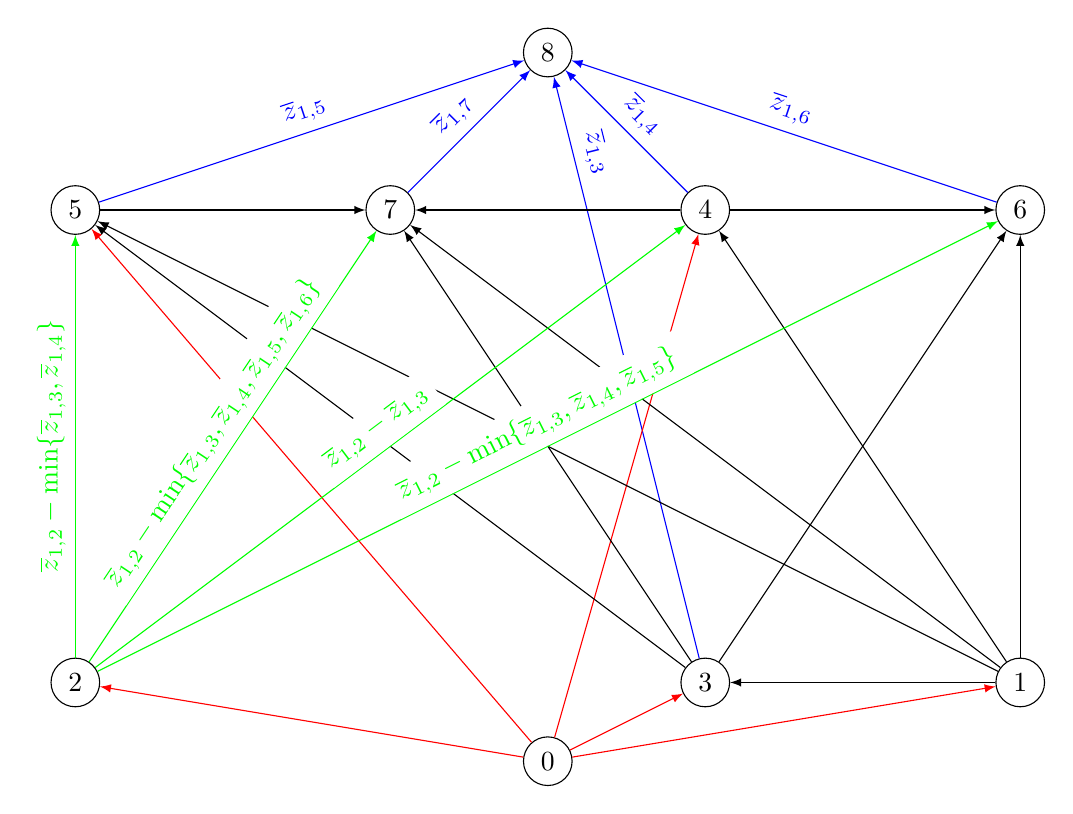
\begin{tikzpicture}
    [  every node/.style={},%
    dot/.style={circle,fill=black,minimum size=4pt,inner sep=0pt,%
      outer sep=-1pt},
    cross/.style={path picture={ 
        \draw
        (path picture bounding box.south east) -- (path picture
        bounding box.north west) (path picture bounding box.south
        west) -- (path picture bounding box.north east); 
      }}]
    \tikzstyle{sommet}=[draw,circle,minimum width=0.5cm]
    \node[sommet] (O) at (0,0) {$0$};
    \node[sommet] (U) at (6,1) {$1$}; 
    \node[sommet] (D) at (-6,1) {$2$}; 
    \node[sommet] (T) at (2,1) {$3$}; 
    \node[sommet] (Q) at (2,7) {$4$}; 
    \node[sommet] (C) at (-6,7) {$5$}; 
    \node[sommet] (Si) at (6,7) {$6$}; 
    \node[sommet] (Se) at (-2,7) {$7$};
    \node[sommet] (H) at (0,9) {$8$};
    
    \draw[->,>=latex,blue] (T) --  node[pos= 0.86,sloped, above] {$
      \overline{z}_{1,3}$} (H) ;
    \draw[->,>=latex,blue] (Q) -- node[sloped,above] {$
      \overline{z}_{1,4}$} (H) ; 
    \draw[->,>=latex,blue] (C) --  node[sloped,above] {$
      \overline{z}_{1,5}$}(H) ; 
    \draw[->,>=latex,blue] (Si) -- node[sloped,above]
    {$ \overline{z}_{1,6}$} (H)  ;
    \draw[->,>=latex,blue] (Se)  -- node[sloped,above] {$
      \overline{z}_{1,7}$} (H) ;
    
    \draw[->,>=latex,red] (O) -- (U);
    \draw[->,>=latex,red] (O) -- (D);
    \draw[->,>=latex,red] (O) -- (T);
    \draw[->,>=latex,red] (O) -- (Q);
    \draw[->,>=latex,red] (O) -- (C);
    
    \draw[->,>=latex] (U) -- (T) ;
    \draw[->,>=latex] (U) -- (Q) ;
    \draw[->,>=latex] (U) -- (C) ;
    \draw[->,>=latex] (U) -- (Si) ;
    \draw[->,>=latex] (U) -- (Se) ;
    
    \draw[->,>=latex] (T) -- (C) ;
    \draw[->,>=latex] (T) -- (Si) ;
    \draw[->,>=latex] (T) -- (Se) ;
    
    \draw[->,>=latex] (Q) -- (Si) ;
    \draw[->,>=latex] (Q) -- (Se) ;
    
    \draw[->,>=latex] (C) -- (Se) ;
    
    \draw[->,>=latex,green] (D) --node[fill=white,sloped,above]
    {$ \overline{z}_{1,2} - \overline{z}_{1,3}$} (Q) ;
    \draw[->,>=latex,green] (D) -- node[fill=white,sloped,above]
    {$ \overline{z}_{1,2} -
      \min\{\overline{z}_{1,3},\overline{z}_{1,4}\}$}(C) ; 
    \draw[->,>=latex,green] (D) -- node[fill=white,sloped,above]
    {$ \overline{z}_{1,2}-
      \min\{\overline{z}_{1,3},\overline{z}_{1,4},\overline{z}_{1,5}\}$}(Si) 
    ; 
    \draw[->,>=latex,green] (D) -- node[fill=white,sloped,above]
    {$
      \overline{z}_{1,2}-\min\{\overline{z}_{1,3},\overline{z}_{1,4},\overline{z}_{1,5},\overline{z}_{1,6}\}$}(Se)
    ; 
    
  \end{tikzpicture}
  \caption{Création du graphe de l'algorithme de séparation pour les
      inégalités de non préemption}
    \label{fig:algo_sep}
  \end{figure}
\end{ex}

Pour séparer un vecteur $\overline{z}_i \in \mathbb{R}^{\E^*}$, nous
calculons un plus long chemin dans le graphe à l'aide de la
programmation dynamique. Pour cela, nous calculons, pour chaque $v \in
\{1,\dots,2n-1\}$, la valeur de du plus long chemin jusqu'à ce somment
$F(v)$ de la manière suivante:
\begin{equation}
  F(v) = \max\{ F(u) + cost (u,v) \ : \ u=1,\dots,v-2 \}
\end{equation}
avec $F(1)=F(2)=0$. 

Puis, on ajoute à ce plus long chemin, la valeur de l'arc servant à
rejoindre le puits. Cela revient à ajouter $\overline{z}_{i,v}$ à
chaque $F(v)$. Si cette valeur est supérieure à celle du
plus long chemin trouvé jusqu'à maintenant, nous remplaçons le plus
long chemin et sa valeur par le nouveau chemin trouvé.

\begin{ex}
Considérons le vecteur $\overline{z}_1$ suivant: $(0,2\, ;\, 0\, ;\,
0,4\, ;\, 0,6\, ;\, 0,6\, ;\, 0\, ;\, 1\, ;\, 0,2)$.

Nous avons $F(1)=F(2)=0$. En effet, l'inégalité devant comporter au moins
trois éléments, $F(1)$ et $F(2)$ ne pourront conduire à une telle
inégalité. La longueur du plus long chemin est initialisée à $0$ et
correspond au chemin vide. De plus,nous avons: 
\begin{itemize}
\item $F(3) =  F(1) + cost (1,3) = F(1) + \overline{z}_{1,1} -
  \overline{z}_{1,2} = 0 + 0,2 - 0= 0,2 $. 
  
  Si nous calculons $F(3)+\overline{z}_{1,3}=0,2+0,4=0,6$. La
  longueur du plus long chemin est donc mise à jour et vaut
  $0,6$. Cette valeur correspondant au chemin $\{1,2,3\}$.
\item $\begin{aligned}[t] 
    F(4) &=  \max \left\{
        \begin{array}{lcl}
          F(1) + cost (1,4) & = & F(1) + \overline{z}_{1,1}  -
                              \min\{\overline{z}_{1,2},\overline{z}_{1,3}\}  \\
          F(2) + cost (2,4) &= & F(2) + \overline{z}_{1,2} -
                              \overline{z}_{1,3}     
        \end{array} \right.\\
    &=  \max \left\{ 
        \begin{array}{lcl}
          0 + 0,2 - 0 &=& 0,2\\
          0 + 0 - 0,4 &= &-0,4 
        \end{array} \right.\\
    &=  0,2
  \end{aligned}$

  Et $F(4)+\overline{z}_{1,4}=0,2+0,6=0,8$. La
  longueur du plus long chemin est donc mise à jour et vaut
  $0,8$. Cette valeur correspondant au chemin $\{1,2,4\}$.

\item $\begin{aligned}[t] 
    F(5) &=  \max \left\{
        \begin{array}{lcl}
          F(1) + cost (1,5) & = & F(1) + \overline{z}_{1,1}  -
                                  \min\{\overline{z}_{1,2},\overline{z}_{1,3},\overline{z}_{1,4}\} 
          \\ 
          F(2) + cost (2,5) &= & F(2) + \overline{z}_{1,2} -
                             \min\{\overline{z}_{1,3}, \overline{z}_{1,4}\}\\
          F(3) + cost (3,5) &= & F(3) + \overline{z}_{1,3} -
                             \overline{z}_{1,4} \\
        \end{array} \right.\\
      &=  \max \left\{ 
        \begin{array}{lcl}
          0 + 0,2 - 0 &=& 0,2 \\
          0 + 0 - 0,4 &= &-0,4 \\
          0,2 + 0.4 - 0,6 &= & 0 \\ 
        \end{array} \right.\\
    &=  0,2
  \end{aligned}$

  Si nous calculons $F(5)+\overline{z}_{1,5}=0,2+0,6=0,8$. Le plus
  long chemin n'est donc pas mis à jour. 

\item $F(6)= 0.2$ et $F(6)+\overline{z}_{1,6}=0,2+0=0,2$. Le plus cours 
  chemin n'es pas mis à jour. 
\item $F(7) = F(4) +\overline{z}_{1,4} -
  \min\{\overline{z}_{1,5},\overline{z}_{1,6}\}= 0,2 + 0,6 - 0 =
  0,8$. De plus, $F(7)+\overline{z}_{1,7}=0,8+1=1,8$. La longueur du
  plus long est donc mise à jour et vaut $1,8$ et correspond au chemin $\{1,2,4,6,7\}$
\end{itemize}

{\'A} la fin de la procédure, le plus long chemin trouvé est donc
$\{1,2,4,6,7\}$ et l'inégalité correspondante, i.e. celle qui sera
ajoutée au modèle, est:
\[  z_{1,1} - z_{1,2} + z_{1,4} - z_{1,6} + z_{1,7} \le 1  \]
\end{ex}  

\subsubsection{Modèles Start/End}
\textcolor{red}{\LARGE pour ce paragraphe => que le texte}
Dans ce paragraphe, nous présentons les résultats obtenus pour le
modèle Start/End.  Les expérimentations ont été conduites
sur les quatre familles d'instances présentées dans le
paragraphe~\ref{sec:instance_CECSP} et avec une limite de temps de
1000 secondes. Le modèle, avec pour objectif la minimisation de la
consommation totale de ressource est utilisé
pour résoudre les instances. Le
tableau~\ref{tab:SE_CECSP} présente ces résultats.

Dans ce tableau, nous avons comparé la qualité et le temps d'obtention
des premières solutions pour chaque famille d'instances testées. Nous
avons aussi comparé le temps nécessaire à l'obtention de la 
solution optimale (1000 secondes si la solution trouvé n'est pas
optimale), la qualité de la solution, le nombre d'instances résolues
et le nombre d'entre elles résolues à l'optimal.

\begin{table}[!htb]
  \begin{center}\small
    \begin{tabularx}{\linewidth}{|Y|YY|YYYY|YY|YYYY|}
      \hline
      \multirow{2}{*}{\#act.} & \multicolumn{2}{c|}{$1^{ère}$ sol.}&
      \multicolumn{4}{c|}{final sol.} & \multicolumn{2}{c|}{$1^{ère}$ 
        sol.}&
      \multicolumn{4}{c|}{sol. finale} \\ 
      \cline{2-13} 
                               & tps(s) & gap & tps & gap  &  \%opt.&\%solv.&
                                                                 tps
                                                                 & gap
                                                                 &
                                                                 tps
                                                                 & gap
                                                                 &
                                                                 \%opt. &\%solv.  \\ 
      \hline
      \multicolumn{7}{|l|}{Famille 1} & \multicolumn{6}{|l|}{Famille 2}\\
      \hline
      $10 $&$ 0,058 $&$ 38 $&$ 45 $&$ 2,9$ &$ 60 $&$ 100$ &$ 0,075 $&$ 24 $&$ 100 $&$ 5,6$ &$ 0 $&$ 100$ \\ 
      $20 $&$ 0,25 $&$ 17 $&$ 100 $&$ 8,4$ &$ 0 $&$ 100$ & $ 0,37 $&$ 8,8 $&$ 100 $&$ 6,5$ &$ 0 $&$ 100$\\ 
      $25 $&$ 0,88 $&$ 21 $&$ 100 $&$ 9,4$ &$ 0 $&$ 100$ &$ 2 $&$ 12 $&$ 100 $&$ 5,8$ &$ 0 $&$ 100$ \\ 
      $30 $&$ 1,3 $&$ 35 $&$ 100 $&$ 10$ &$ 0 $&$ 100$&$ 3,1 $&$ 14 $&$ 100 $&$ 6,3$ &$ 0 $&$ 100$  \\ 
      \hline   
      \multicolumn{7}{|l|}{Famille 3} &  \multicolumn{6}{|l|}{Famille 4}\\
      \hline 
    $10 $&$ 0,064 $&$ 4,1 $&$ 64 $&$ 1,8$ &$ 40 $&$ 100$ &$ 0,037 $&$ 0 $&$ 0,037 $&$ 0$ &$ 100 $&$ 100$\\ 
$20 $&$ 2,8 $&$ 6,8 $&$ 100 $&$ 3,9$ &$ 0 $&$ 100$ &$ 0,61 $&$ 0,72 $&$ 0,63 $&$ 0$ &$ 100 $&$ 100$\\ 
$25 $&$ 17 $&$ 4,5 $&$ 100 $&$ 4,5$ &$ 0 $&$ 100$ &$ 1,5 $&$ 0,31 $&$ 1,5 $&$ 0$ &$ 100 $&$ 100$\\ 
$30 $&$ 24 $&$ 6,4 $&$ 100 $&$ 4,1$ &$ 0 $&$ 80$ &$ 4,8 $&$ 0,07 $&$ 15 $&$ 0$ &$ 89 $&$ 89$ \\ 
      \hline 
    \end{tabularx}
  \end{center}
  \caption{Résultats du PLNE indexé par le temps du \CECSP~avec et
    sans coupes énergétiques.} 
  \label{tab:SE_CECSP}
\end{table}

\subsubsection{Modèles On/Off}

\paragraph{Résultats du modèle On/Off pour le \CECSP}
Dans ce paragraphe, nous présentons les résultats obtenus pour le
modèle On/Off. Les expérimentations conduites pour ce modèle dans le
cadre du \CECSP~l'ont été
sur les instances de la Famille 4 (cf. tableau~\ref{tab:OO_f4}) et sur les
instances de la Famille 1 (cf. tableau~\ref{tab:OO_f1}) avec une
limite de temps de 1000 secondes.  

Pour la Famille 4, le tableau~\ref{tab:OO_f4} présente le pourcentage
d'instances résolues à l'optimal ainsi que le temps nécessaire à leur 
résolution pour différentes combinaisons de coupes ajoutées au
modèle. Dans le tableau, ces différentes inégalités sont représentées
de la manière suivantes: 
\begin{itemize}
\item {\it Sep.} ou {\it S.} représente les inégalités
 bornant supérieurement la distance entre deux événements;
\item {\it Date} ou {\it D.} les inégalités bornant supérieurement la
  date des événements;
\item {\it SàD} les inégalités déduites du problème du sac-à-dos
  (cf. paragraphe~\ref{sec:maxDist}), et  
\item {\it $\overline{Preem.}$} ou {\it $\overline{P.}$} les
  inégalités de non-préemption (cf. paragraphe~\ref{sec:nonPreem}).
\end{itemize}
 Les deux premiers ensembles d'inégalités sont ajoutés directement
 dans le modèle et sont aussi utilisées comme borne plus fine dans les
 contraintes du modèle (voir paragraphe~\ref{sec:maxDist}).


\begin{table}[!htb]
  \begin{center} 
    \begin{tabular}{|c|>{\centering\arraybackslash}p{1cm}>{\centering\arraybackslash}p{1cm}|>{\centering\arraybackslash}p{1cm}>{\centering\arraybackslash}p{1cm}|>{\centering\arraybackslash}p{1cm}>{\centering\arraybackslash}p{1cm}|>{\centering\arraybackslash}p{1cm}>{\centering\arraybackslash}p{1cm}|}
      \hline
      \multirow{2}{*}{\backslashbox{ineg.}{\#act.}}  &
                                                        \multicolumn{2}{c|}{10} & \multicolumn{2}{c|}{20} & \multicolumn{2}{c|}{25} & \multicolumn{2}{c|}{30}\\
      & tps(s) & \%opt & tps(s) & \%opt& tps(s) & \%opt& tps(s) & \%opt\\
      \hline
     $Aucune$ & $ 0,3 $&$ 100 $&$ 164,14 $&$ 90,9 $&$ 635,4 $&$ 55,6 $&$ 968 $&$ 10$\\
     $ Sep.$ &$ 0,6 $&$ 100 $&$ 182,2$&$ 90,9 $&$ 727,3 $&$ 55, 6 $&$ 851$&$ 20$ \\
     $ Date $&$ 0,5 $&$ 100 $&$ 167,3 $&$ 90,9 $&$ 629,5$&$ 88,9 $&$ 961,4$&$ 20 $\\
     $ SàD$&$ 0,5 $&$ 100 $&$ 164,7 $&$ 90,9 $&$ 555,1$&$ 66,7 $&$ 845,3$&$ 20 $\\
     $ \overline{Preem.}$ &$ 0,3$&$ 100 $&$ 330,9 $&$ 72,7 $&$ 822,4 $&$ 44,4 $&$ 914,8$&$ 10$ \\
     %$ Sep\ \$&$\ Date $$&$ 100 $&$ $&$ 90,9 $&$ $&$ 66,7 $&$ $&$ 10 \\
     %$ Sep\ \$&$\ SàD$$&$ 100 $&$ $&$ 81,8 $&$ $&$ 77,8 $&$ $&$ 20 \\
     %$ Sep\ \$&$\ \overline{Preem.}$ $&$ $&$ 100 $&$ $&$ 81,8 $&$ $&$ 33,3 $&$ $&$ 10 \\
     %$ Date\ \$&$\ SàD$$&$ 100 $&$ $&$ 90,9$&$ 88,8 $&$ $&$ 10\\
     %$ Date\ \$&$\ \overline{Preem.}$ $&$100 $&$ $&$ 81,8 $&$ $&$ 66,7 $&$ $&$ 20 \\ 
     %$ SàD\ \$&$\ \overline{Preem.}$ $&$ $&$ 100 $&$ $&$ 90,9 $&$ $&$ 33, 3 $&$ $&$ 10\\
     $ I.\ \&\ T.\ \&\ SàD$&$ 0,6 $&$100 $&$ 154$&$ 90,9 $&$ 389,9 $&$ 77,8 $&$ 839,9$&$ 20$\\
     $ I.\ \&\ T.\ \&\ \overline{P.}$ &$ 0,6 $&$ 100 $&$ 179,8 $&$ 90,9 $&$
                                                                   454,4 $&$ 77,8 $&$ 813,8$&$ 60$ \\
     $ I.\ \&\ SàD\ \&\ \overline{P.}$&$ 0,5 $&$100 $&$ 182,2$&$ 90,9 $&$759,6 $&$ 33,3 $&$ 924,9$&$ 20$\\
     $ T.\ \&\ SàD\ \&\ \overline{P.} $&$ 0,5$&$ 100 $&$ 170$&$ 90,9 $&$ 705$&$ 66,7 $&$ 816$&$ 50$\\
     $ I.\ \&\ T.\ \&\ SàD\ \&\ \overline{P.}$&$ 0,9 $&$ 100 $&$ 278,9 $&$ 81,8 $&$ 510$&$ 88,9 $&$ 802,8$&$ 50$\\
      \hline
    \end{tabular}
  \end{center}
  \caption{Résultats du modèle On/Off pour le \CECSP~avec différentes
    combinaisons de coupes (Famille 4).}
  \label{tab:OO_f4}
\end{table}

Dans le tableau~\ref{tab:OO_f4}, nous pouvons remarquer que le nombre
d'instances à $10$ et $20$ activités résolues est du même ordre de
grandeur pour toutes les combinaisons d'inégalités testées. Pour les
instances à $25$ activités, les résultats sont plus hétérogènes mais
les meilleures résultats sont obtenus en combinant toutes les
inégalités. Enfin, pour les instances à $30$ activités, les meilleurs
résultats sont quant à eux obtenus en combinant seulement inégalités
de non-préemption et les deux ensembles d'inégalités portant sur les
dates des événements, i.e. {\it Sep} et {\it Date}. Cependant, les
résultats obtenus en combinant toutes les inégalités ne sont pas très
éloignés de ceux obtenant les meilleurs résultats.

Pour les instances de la Famille 1, seulement un petit nombre
d'instances sont résolues de manière optimale. C'est pourquoi nous
présentons seulement le pourcentage d'instances pour lesquelles une
solution a été trouvée et nous calculons la distance entre cette
solution et la meilleure borne inférieure trouvée à la fin du temps
imparti. Ces résultats sont présentés dans le
tableau~\ref{tab:OO_f1}. Les notations sont les mêmes que celles
utilisées dans le tableau~\ref{tab:OO_f4}.

\begin{table}
  \begin{center} 
    \begin{tabular}{|c|>{\centering\arraybackslash}p{1cm}>{\centering\arraybackslash}p{1.2cm}|>{\centering\arraybackslash}p{1cm}>{\centering\arraybackslash}p{1cm}|>{\centering\arraybackslash}p{1cm}>{\centering\arraybackslash}p{1cm}|>{\centering\arraybackslash}p{1cm}>{\centering\arraybackslash}p{1cm}|}
      \hline
      \multirow{2}{*}{\backslashbox{ineg.}{\#act.}}  &
                                                        \multicolumn{2}{c|}{10} & \multicolumn{2}{c|}{20} & \multicolumn{2}{c|}{25} & \multicolumn{2}{c|}{30}\\
      & \%feas. & gap &\%feas. & gap& \%feas. & gap& \%feas. & gap\\
      \hline
      $ Aucune$ &$ 100 $&$ 23,2 $&$ 81,8 $&$ 74,5 $&$ 22,2 $&$ 91,9 $&$ 0 $&$ 0$\\
      $ Sep$ &$ 100 $&$ <0,01 $&$ 100 $&$ 14,9 $&$ 44,4 $&$ 68,9 $&$ 0 $&$ 0$\\
      $ Date $ &$100$&$ 1,06 $&$ 100 $&$ 70,5 $&$ 33,3$&$ 88,1 $&$ 40$&$ 84,9 $\\
      $ SàD$ &$ 100 $&$ 9,8 $&$ 100 $&$ 46,4 $&$ 77,78 $&$ 64,6 $&$ 25$&$ 70,7 $\\
      $ \overline{Preem.}$ &$ 100 $&$ 61,5 $&$ 81,8 $&$ 73,4 $&$ 0 $&$ 0 $&$ 0 $&$ 0$\\
      $ S.\ \&\ D.\ \&\ SàD$&$ 100 $&$<0,01 $&$ 100$&$ 13,7 $&$ 100 $&$ 51,5 $&$ 50$&$ 70,6$\\
      $ S.\ \&\ D.\ \&\ \overline{P.}$ &$ 100 $&$ 4,77 $&$ 100 $&$ 45,5 $&$
                                                                   88,89 $&$ 75,1 $&$ 30$&$ 84,6 $\\
      $ S.\ \&\ SàD\ \&\ \overline{P.}$ &$ 100 $&$ 8,67 $&$ 100 $&$ 68,3 $&$
                                                                   44,4
                $&$ 88,1 $&$ 10 $&$ 93$\\
     $ D.\ \&\ SàD\ \&\ \overline{P.}$ &$ 100$&$ 23,8 $&$ 100$&$ 60,1 $&$ 83,3$&$ 79,8 $&$ 30$&$ 88,2$\\
     $ S.\ \&\ D.\ \&\ SàD\ \&\ \overline{P.}$ &$ 100 $&$ 0,07 $&$ 100 $&$ 35,7 $&$ 100$&$ 66,9 $&$ 10$&$ 87,1$\\
      \hline
    \end{tabular}
  \end{center}
  \caption{Résultats du modèle On/Off pour le \CECSP~avec différentes
    combinaisons de coupes (Famille 1).}
  \label{tab:OO_f1}
\end{table}

Dans le tableau~\ref{tab:OO_f4}, nous pouvons voir que les meilleurs
résultats sont obtenus en combinant {\it Sep, Date} et {\it
SàD}. Cependant, des résultats comparables sont obtenus en combinant
{\it Sep, Date} et {\it $\overline{Preem.}$} ou {\it Sep, Date, SàD} et
{\it $\overline{Preem.}$}.


\paragraph{Résultats du modèle On/Off pour le \RCPSP}

Nous allons maintenant évaluer les performances relatives des
améliorations du modèle On/Off dans le cadre du \RCPSP. Pour ce faire,
les expérimentations ont été conduites sur les instances de Kone {\it
et al}~\cite{modele_RCPSP} et décrites dans le
paragraphe~\ref{sec:instances_RCPSP} avec un pré-calcul des fenêtre de
temps des activités aussi décrit dans le
paragraphe~\ref{sec:instances_RCPSP}. La limite de temps est fixée à
1000 secondes.

Pour ces instances, le tableau~\ref{tab:OO_PSP} présente le
pourcentage d'instances résolues à l'optimal ainsi que le temps
nécessaire à leur résolution pour différentes combinaisons de coupes
ajoutées au modèle. 

\begin{table}[!htb]
 \begin{center}
   \begin{tabular}{|c|cc|ccc|}
     \hline
       \multirow{2}{*}{\backslashbox{ineg.}{\#act.}} & \multicolumn{2}{c|}{$1^{ère}$ sol.}& \multicolumn{3}{c|}{Sol. finale}\\ 
	\cline{2-6}
     & time(s) & gap & time & gap &\%opt  \\ 
 \hline 
     $Aucune$ &$0,19$& $3,4 $&$ 34,8$ &$ 0 $& $100$\\
     $Sep.$ & $0,17 $& $3,2 $&$ 30,3$ &$ 0 $& $100$ \\ 
     $\overline{Preem.}$ & $0,17 $&$ 3,8$& $30,3$ & $0 $& $100 $ \\ 
     $Sep.\ \&\ \overline{Preem.}$ & $0,29$& $3,3$ & $ 33,1 $& $0$ & $100$ \\ 
\hline 
\end{tabular}
\end{center}
  \caption{Résultats du modèle On/Off pour le \RCPSP~avec différentes
    combinaisons de coupes.}
  \label{tab:OO_PSP}
\end{table}

Dans le tableau~\ref{tab:OO_PSP}, nous pouvons voir que les résultats
de l'ajout des coupes et inégalités a moins d'impact dans le cadre du
\RCPSP. Cependant, une amélioration des performances du modèle,
spécialement pour l'ajout des inégalités {\it Sep.} ou {\it
  $\overline{Preem.}$}, peut être notée. Cette amélioration est
moindre dans le cas où les deux ensembles d'inégalités sont ajoutés
simultanément. 

\subsection{Comparaison des différentes approches}

Dans ce paragraphe, nous allons effectuer des comparaisons entre
différentes des méthodes décrites ci-dessus. Dans un premier temps et
pour montrer que dans certains cas, le modèle indexé par le temps peut
produire des solutions sous-optimales, nous comparons les résultats de
ce dernier avec ceux du modèle On/Off (sans ajout de coupes
particulières) sur la Famille d'instances 1.   

Le tableau~\ref{CECSPMIPOBJ} présente ces résultats. Pour chacune des
formulation, la première colonne décrit le temps passé dans la
résolution du PLNE. La seconde colonne représente le pourcentage
d'instances résolues à l'optimal et la troisième colonne le nombre
d'instances pour lesquelles une solution réalisable a été
trouvé. Enfin, la dernière colonne du tableau montre la différence
moyenne entre la valeur de l'objectif retourné par les deux
modèles. Par exemple, la première valeur de cette colonne nous dit
que, pour les instances à $20$ activités, la valeur de l'objectif
retourné par le modèle indexé par le temps est, en moyenne, $10\%$
plus élevée que celle retournée par le modèle à événements. 

\begin{table}[ht] \centering
  \begin{tabular}{|c|ccc|ccc|c|}
    \hline
    & \multicolumn{3}{c|}{Modèle On/Off} &  \multicolumn{3}{c|}{Modèle
                                           indexé par le temps} &\\
    \hline
    \#act.&tps(s)&\%optimal&\%feas.&tps(s)&\%optimal
                              &\%feas.&\%dev. obj. \\
    \hline
    20 &7200 &0 &100 &7200 &0 &100 & 10,08\\
    25 &7200 &0 &44,44 &7200 &0 &66,67 & 10,11\\
    \hline
  \end{tabular}
  \caption{Comparaison du modèle On/Off et du modèle indexé par le
    temps pour le \CECSP.}
  \label{CECSPMIPOBJ}
\end{table}

Tout d'abord, nous pouvons remarquer que le modèle indexé par le temps
permet de trouver une solution réalisable pour plus d'instances que le
modèle On/Off. Cependant, aucun des deux modèles n'est capable de
résoudre les instances de manière optimale. Enfin, le modèle On/off
trouve clairement de meilleures solutions que le modèle indexé par le
temps. 

Les modèles présentés dans ce manuscrit ont de grandes difficultés à
trouver des solutions optimales. En particulier lorsque des fonctions
de rendement, même seulement affines, entrent en jeu. De plus, les
méthodes testées dans le paragraphe suivant, portant sur les techniques
issues de la programmation par contraintes, ne le sont que pour la
variante décisionnelle du \CECSP, i.e. sans objectif. De ce fait, nous
allons présenter les résultats des trois différents modèles dans le
cas où aucun objectif n'est présent. Le tableau~\ref{MIPresult}
présente ces résultats. 

Pour chacun des modèles, trois colonnes exposent les résultats. La
première correspond au temps nécessaire pour trouver une solution (si
une solution est trouvée). La seconde correspond au pourcentage
d'instance résolue et la dernière colonne correspond au nombre
d'instances prouvée réalisable. Cette dernière colonnes est introduite
pour permettre de montrer que le modèle indexé par le temps peut
prouver l'infaisabilité de l'instance alors que les modèles a
événements trouve une solution pour cette même instance et qu'elle est
donc réalisable. De ce fait, le modèle indexé par le temps
sur-contraint bien le problème initial. 

\begin{table}[ht] \centering
  \begin{tabular}{|c|ccc|ccc|ccc|}
\hline & \multicolumn{3}{c}{Indexé par le tps} & \multicolumn{3}{|c}{On/off} & \multicolumn{3}{|c|}{Start/End}\\ \hline
\#act. & tps (s) & \%solv. &
\%feas. & tps(s) & \%solv. &
\%feas. & tps(s) & \%solv. &
\%feas. \\ \hline 
    \multicolumn{10}{|c|}{Famille 1}\\
    \hline
   $ 10	$&$	0.03	$&$	100	$& $60$& $0,22$ & $100$ & $100$&$	0,71	$&$	100	$&$	100$	\\
   $ 20	$&$	0,08	$&$	100	$&$	54,5	$& $11,57$ & $100$ & $100$&$	355,4	$&$	100	$&$	100$	\\
    $25	$&$	0,22	$&$	100	$&$	66,7	$&$58,79$ & $100$ & $100	$&$	2226,7	$&$	77,8	$&$	77,8$	\\
    $30	$&$	0,25	$&$	100	$&$	60	$& $1582,9$ &
                                                                     $80$ & $80 $&$	6247,2	$&$	20	$&$	20$	\\
    $60	$&$	420	$&$	100	$&$	100	$&$4969,51$ & $80$ & $80	$&$	6219,8	$&$	20	$&$	20$	\\
    \hline 
    \multicolumn{10}{|c|}{Famille 3}\\
    \hline
   $ 10	$&$	0,04	$&$	100	$&$	100	$&$0,46$ & $100$ & $100$&$0,88	$&$	100	$&$	100$	\\
   $ 20	$&$	0,24	$&$	100	$&$	100	$&$658,362$ & $100$ & $100$&$	1430,6	$&$	90,9	$&$	90,9$	\\
   $ 25	$&$	0,45	$&$	100	$&$	88,9	$&$	1900,17$ & $77,78$ & $77,78	$&$	5816,1	$&$	33,3	$&$	33,3$	\\
   $ 30	$&$	1,38	$&$	100	$&$	100	$&$	2819,7$ & $80$ & $80$&$	6011,8	$&$	20	$&$	20$	\\
  $  60	$&$	328,7	$&$	100	$&$	80	$&$6358,15$ & $20$ & $20$&$	7200	$&$	0	$&$	0$	\\
    \hline 
    \multicolumn{10}{|c|}{Famille 4}\\
    \hline
   $ 10	$&$	0,01	$&$	100	$&$	100	$&$	0,23	$&$	100	$&$	100	$&$	0,7	$&$	100	$&$	100$	\\
  $  20	$&$	0,27	$&$	100	$&$	100	$&$	734,04	$&$	90,9	$&$	90,9	$&$	2995,9	$&$	63,6	$&$	63,6$	\\
   $ 25	$&$	0,7	$&$	100	$&$	100	$&$	2102,85	$&$	77,8	$&$	77,8	$&$	4833,6	$&$	44,4	$&$	44,4$	\\
   $ 30	$&$	1,57	$&$	100	$&$	100	$&$	4483,4	$&$	60	$&$	60	$&$	6485,9	$&$	20	$&$	20$	\\
   $ 60	$&$	224,72	$&$	100	$&$	60	$&$	7200	$&$	0	$&$	0	$&$	7200	$&$	0	$&$	0$	\\
    \hline
  \end{tabular}
  \caption{Comparaison des trois modèles de PLNE du \CECSP~sans
    fonction objectif.}
  \label{MIPresult}
\end{table} 

Comme nous pouvons le voir dans le tableau~\ref{MIPresult}, le
modèle indexé permet de trouver des solutions beaucoup plus rapidement
que les modèles à événements. Cependant, ce modèle ne peut être
employé comme une méthode de résolution exacte  puisque, pour
certaines instances, seules des solutions fractionnaires existent. 

Parmi les deux formulations basées sur les événements, la formulation
On/Off est celle qui fournie les meilleurs résultats en termes de
temps de calcul et de nombre d'instances résolues. 
